% PEX_KERNEL_REVISION_MAIN
\documentclass[conference,9pt,letterpaper]{IEEEtran}
\usepackage[T1]{fontenc}
\usepackage{amsmath,amssymb,graphicx,booktabs,array,microtype}
\usepackage[hidelinks]{hyperref}
\usepackage[ruled,vlined,linesnumbered]{algorithm2e}
\SetKwInOut{Input}{Input}
\SetKwInOut{Output}{Output}
\DontPrintSemicolon
\SetAlFnt{\scriptsize}
\SetAlCapFnt{\footnotesize}
\SetAlCapNameFnt{\footnotesize}
\SetAlgoNlRelativeSize{-1}

\hypersetup{pdfauthor={},pdftitle={CapFill: Learned Capacitance Estimation from Sparse Characterization for Pattern-Based Parasitic Extraction}}
\newcommand{\nrmse}{\operatorname{NRMSE}}
\title{CapFill: Learned Capacitance Estimation from Sparse Characterization for Pattern-Based Parasitic Extraction}
\author{\IEEEauthorblockN{Anonymous authors}\IEEEauthorblockA{\vphantom{Department and affiliation}\vphantom{City, Country}\\\vphantom{Contact information}}}
\begin{document}
\bstctlcite{dac:bibcontrol}
\maketitle

\begingroup
\renewcommand{\thefootnote}{}
\footnotetext{Anonymous code and reproducibility artifacts are available at\par
\noindent\url{https://anonymous.4open.science/r/capfill-paper-release-8BE6/}}
\endgroup
\begin{abstract}
Pattern-based parasitic extraction relies on pre-characterized capacitance data to evaluate interconnect geometries. With limited characterization, numerical interpolation errors at uncharacterized geometries can affect extracted capacitances and downstream timing analysis. We propose CapFill, an observation-conditioned learning framework for improving capacitance estimation accuracy without increasing the supplied characterization budget. Its main implementation, Full, combines a numerical anchor, Transformer residuals, and applicable numerical corrections through component-wise gating informed by support geometry and candidate agreement. Estimates can be prepared in native compute tables while retaining existing lookup and parasitic-network assembly procedures. A census of 9.89 million OpenRCX calls finds that 55.77\% are raw non-node requests. Across public rules, finite-element data, and cross-process transfer, Full lowers condition-level macro normalized root-mean-square error (NRMSE) relative to the OpenRCX kernel and multilinear interpolation with sparse-support extension in all 60 evaluated conditions spanning 10--70\% characterization holdout. Binary and Ungated outperform both baselines in 55 and 50 conditions, respectively. This empirical consistency motivates Full as CapFill's default implementation, without implying optimality on every condition or downstream metric. Separate fixed-node rule-export experiments improve net-capacitance and worst-slack fidelity relative to both kernel controls in all 16 layout--budget settings. At $B=8$, mean endpoint timing error decreases by 77.8--91.1\% across four IBEX layouts. These evaluations connect learned capacitance estimation under limited characterization to extraction fidelity and timing fidelity.
\end{abstract}

\section{Introduction}
Pattern-based parasitic extraction relies on pre-characterized capacitance data to estimate the electrical response of interconnect geometries encountered during layout extraction. Since only a finite set of geometries can be characterized, numerical interpolation may introduce errors for uncharacterized configurations. These errors can propagate into extracted capacitances and downstream static timing analysis (STA). This work addresses capacitance estimation accuracy under limited characterization budgets.

The pattern-based workflow separates pre-characterization from layout extraction~\cite{tsai}. Representative interconnect patterns and process parameters are first evaluated by a field solver to build a pre-characterized library. During extraction, layout geometries are recognized and matched to patterns, capacitances are obtained by lookup, interpolation, or fitting, and the resulting values are assembled into a parasitic RC network. Increasing characterization density can reduce interpolation error but requires additional reference samples~\cite{yang2023cnncap,zhou2026rmlpcap}. Our focus is the estimation step that connects the available process-specific samples to uncharacterized geometries.

Prior work has automated pattern and formula construction from field-solver samples~\cite{li2020autoprechar}, developed neural capacitance and matrix predictors~\cite{yang2023cnncap,zhou2026rmlpcap,attentioncap,flash}, and studied geometry and layer-thickness exploration~\cite{tsai}. We propose CapFill, an observation-conditioned learning framework that combines real characterization observations, geometry and process context, and a numerical anchor with learned and numerical residual corrections. CapFill retains the field solver as a source of reference characterization and leaves pattern recognition and matching unchanged.

\begin{figure}[t]
\centering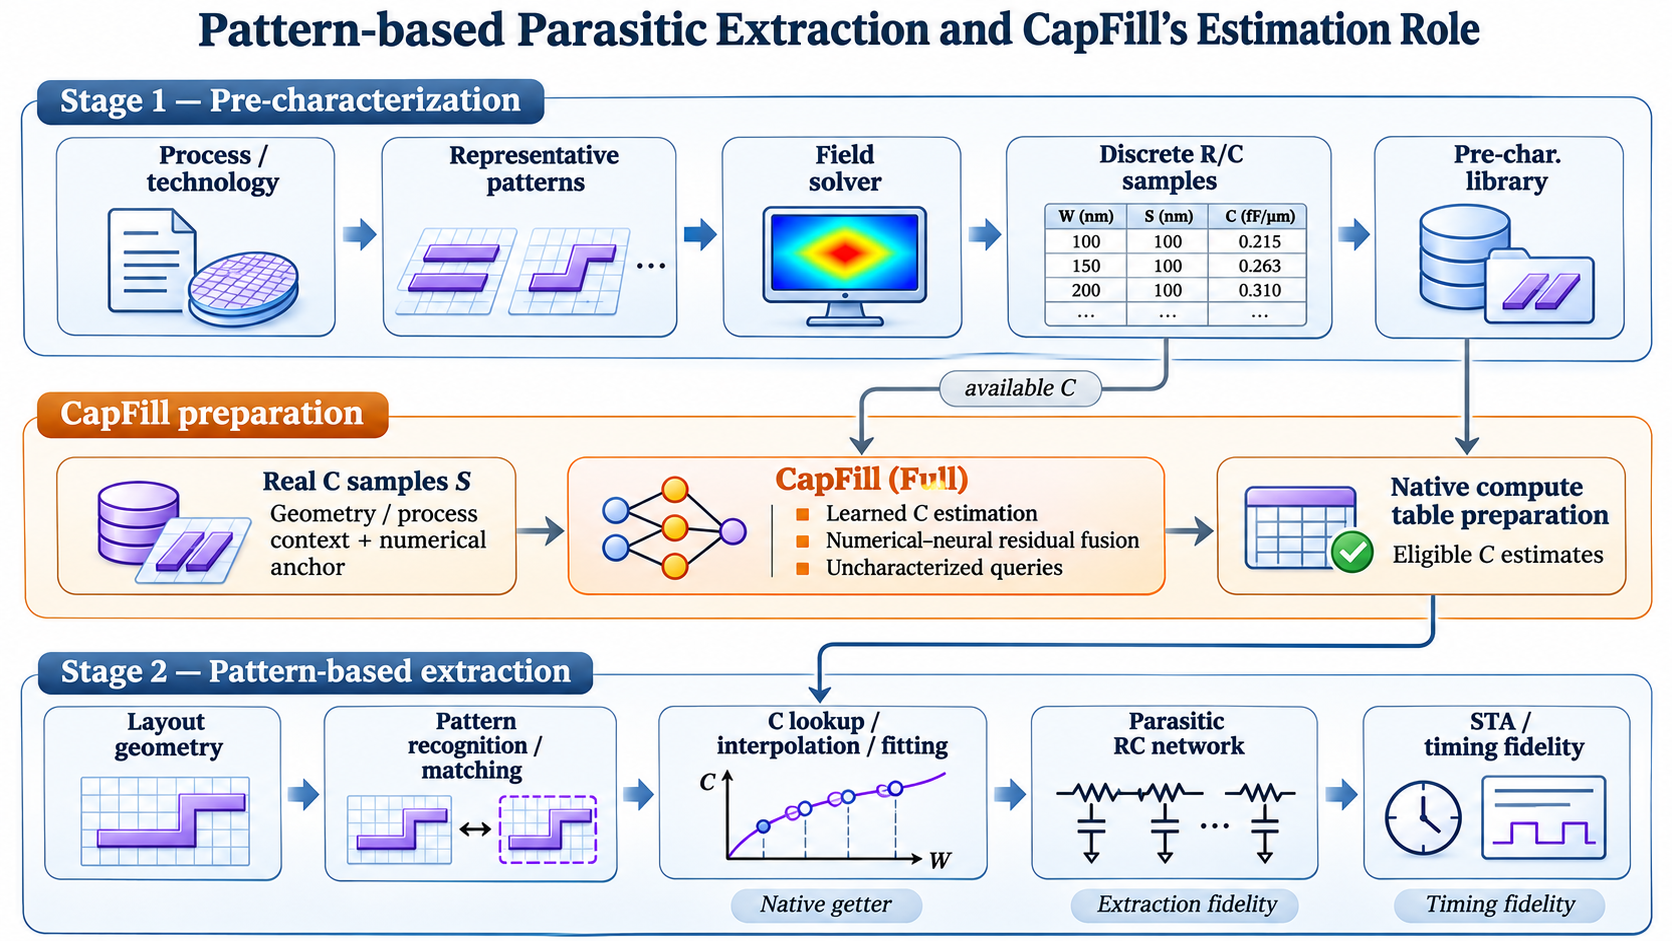
\includegraphics[width=\columnwidth]{figures/pattern_based_capfill_workflow.png}
\caption{Pattern-based parasitic extraction and CapFill's estimation role. The two-stage organization follows the workflow in~\cite{tsai}. The highlighted path shows where CapFill prepares estimates. CapFill uses available real capacitance samples and geometry/process context to estimate uncharacterized capacitances. Eligible estimates are prepared in native compute tables before layout queries. Pattern matching, native getters, and parasitic-network assembly remain unchanged. We evaluate extraction and timing fidelity downstream.}
\label{fig:OpenRCX}
\end{figure}

For a target process and pattern context, observed geometry--capacitance pairs reveal the local electrical response and complement information learned from other characterization data. CapFill conditions on those observations with fixed learned parameters, including when the target has too few observations to fit a flexible model independently. Geometry tokens encode observation indicators, known capacitances, and anchor estimates, while material tokens supply process context. A shared Transformer relates uncharacterized query geometries to the observed response. Full, the main CapFill implementation, uses the complete numerical--neural residual fusion. Binary simplifies the gate, and Ungated removes it.

Our primary contribution is improving capacitance estimation accuracy under limited characterization budgets, with downstream extraction and timing fidelity evaluation. OpenRCX provides a concrete integration setting: its native extraction rules encode process-specific data and are evaluated using coupling distance and surrounding routing context~\cite{orcx_runtime,openrcx}. CapFill estimates can be incorporated into these native data structures during preparation. The existing lookup and parasitic-network assembly procedures then consume the prepared values without neural inference at each layout query. Compute-table preparation is the deployment mechanism for the estimator, while the research objective is accurate capacitance estimation and its downstream effect (Fig.~\ref{fig:OpenRCX}).

We evaluate characterization holdout, observation budgets, cross-process prediction, extraction fidelity, and timing fidelity. Full is the default implementation evaluated alongside its Binary and Ungated ablations.

Our selection objective is consistent improvement over the two traditional kernel baselines across the evaluated conditions. Across public rules, finite-element (FEM) data, and cross-process transfer, Full lowers condition-level macro NRMSE relative to both the OpenRCX kernel and multilinear interpolation with sparse-support extension (MLI-ext.) in all 60 evaluated conditions, spanning different support regions, missingness patterns, and 10--70\% characterization holdout (Fig.~\ref{fig:coverage}). Binary and Ungated outperform both baselines in 55 and 50 conditions, respectively. When it is not known in advance which simplified variant will better suit a target condition, this observed consistency supports Full as a unified default. Binary and Ungated can still be more accurate in individual conditions or on particular downstream metrics. Performance on unseen conditions remains an empirical question.


We introduce CapFill to estimate capacitance from sparse characterization through numerical--neural residual fusion. We integrate its estimates into native compute tables while preserving measured values, resistance, lookup, and RC-network assembly. Matched evaluations connect estimation accuracy under limited budgets to extraction and timing fidelity. We report preparation and extraction costs separately.
%The evaluation retains conditions where numerical or simpler learned methods are better.

\section{Problem and Related Work}
\subsection{Pattern-based extraction and capacitance estimation}
Pattern-based extraction is also described as rule-based or 2.5-D extraction~\cite{tsai}. We use pattern-based extraction for the overall methodology and reserve native extraction rules, rule tables, and compute tables for the OpenRCX implementation.

\textbf{Stage 1: Pre-characterization.} Process and technology parameters define representative interconnect patterns. A field solver supplies discrete resistance/capacitance samples, from which a pre-characterized library is constructed.

\textbf{Stage 2: Pattern-based extraction.} Layout geometry undergoes pattern recognition and matching. Capacitance lookup, numerical interpolation, or fitting supplies electrical values for the matched geometry, and parasitic-network assembly constructs the RC network~\cite{tsai}. Runtime requests may fall between or beyond the characterized geometries.

CapFill improves capacitance estimation at this interface: it uses only available real characterization observations, geometry and process context, and a numerical anchor to estimate uncharacterized values. In our OpenRCX integration, estimates are prepared in eligible native compute-table entries before runtime queries. A native rule is identified by process/corner, pattern family, and layer context. The retained getter performs width selection, coordinate mapping, quantization, and boundary handling. Those implementation choices are part of the evaluated native algorithm.

\subsection{Measured off-grid demand}
Across two instrumented OpenRCX getters on eight unchanged routed layouts, we record 9,888,586 calls and 19,562 unique rule/geometry keys. The calls comprise 2,696,515 node hits, 4,547,424 non-node requests inside the selected width slice, 967,755 outside it, and 1,676,892 fringe/special requests. Raw non-node requests account for 55.77\% of all logged calls and 67.16\% of finite-distance calls (Fig.~\ref{fig:census}). Native width mapping and compute-grid quantization send 849,663 raw non-node requests to effective characterization nodes.

\begin{figure}[t]
\centering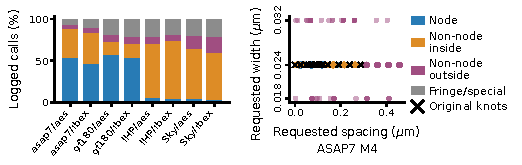
\includegraphics[width=\columnwidth]{figures/query_census.pdf}
\caption{Measured non-node demand. Left: occurrence-weighted query classes over two logged capacitance getters on eight fixed layouts. Right: ASAP7 M4 requests and original knots, with marker area scaled by log occurrence. 
%Counts exclude resistance, five-argument diagonal getters and later assembly; they are neither capacitance nor runtime weights. Raw and effective node identities differ under native mapping.
}
\label{fig:census}
\end{figure}
The trace preserves SPEF electrical records on all layouts. 

% It establishes the frequency of non-node evaluation in these getters, not the fraction of all PEX work. Characterization holdout is a different quantity: it varies the available information rather than measuring runtime request frequency. We evaluate all four requested holdout levels without equating them to the census percentages.

\subsection{Problem formulation and kernel scope}
For context $c$, available observations $S=\{(x_i,y_i)\}$ and query coordinates $Q$, the estimator satisfies
\begin{equation}
\widehat y_Q=F_\theta(S,Q,c),\qquad \widehat y(x_i)=y_i\ (x_i\in S).
\end{equation}
An off-grid geometry need not lie outside support. Inside-support classification requires affine-space and hull membership.
% incompatible topologies or outputs are excluded explicitly. 
Only observed values in $S$ enter prediction. We use query reference values only for scoring.

Commercial platforms such as Siemens Calibre xACT/xACT 3D, Calibre xRC, and Synopsys StarRC are integrated extraction systems~\cite{siemens_calibre_xact,siemens_calibre_xact3d,siemens_calibre_xrc,synopsys_starrc}. Our comparison concerns capacitance-estimation operators within pattern-based extraction, not a ranking of complete commercial products. We use the open-source OpenRCX implementation and a specified MLI operator as reproducible kernel baselines~\cite{openroad_openrcx}.

The primary algorithmic comparison is the pinned OpenRCX finite-distance kernel and specified multilinear interpolation (MLI). Specified MLI implements the mathematical core of supplied Calibre xRC fast interpolation. %This comparison concerns the interpolation operator,
%commercial binaries and product-specific boundary policies are outside its scope. 
Complete cells require $2^d$ vertices, in $d$ dimensions,
\begin{equation}
\widehat y(x)=\sum_{\epsilon\in\{0,1\}^d}y_\epsilon
 \prod_{j=1}^d t_j^{\epsilon_j}(1-t_j)^{1-\epsilon_j}.
\end{equation}
% Sparse-support completion and boundary clamping are separately declared extensions, not attributed to xRC.
Physical data have rank one or two. Four-dimensional evaluation is an implementation test only. OpenRCX comparison retains native width selection, integer geometry and four-unit compute bins. A continuous-distance variant isolates quantization effects. General numerical predictors are component controls.

\subsection{Related models and interfaces}
AttentionCap predicts capacitance matrices from conductor/material tokens~\cite{attentioncap}, whereas Flash-CNNCap predicts window contributions in a three-dimensional DEF-to-SPEF workflow~\cite{flash}. 
AttentionCap itself supports partial matrix-row supervision. Our component-supervised AttentionCap adaptation tests a specified observation budget and fitting recipe.
% rather than a general limit of matrix architectures. 
Flash-CNNCap's 3D window task is not converted into a mismatched 2D speed ranking.
ResCap corrects initial physical estimates~\cite{rescap}, while hybrid PEX selects extraction methods by window~\cite{hybrid}. Here the anchor uses current observations and fusion acts within a rule. CNPs~\cite{cnp} and attentive neural processes~\cite{anp} provide conditional regression interfaces.
%not categorized as a field solver.

% \section{Estimator and Compute-Table Preparation}
% % \subsection{Observation-conditioned residual fusion}
% % The anchor uses piecewise-linear interpolation for rank-one support, simplex interpolation inside higher-rank support, and nearest-observation fallback outside or for degeneracy. Tokens encode geometry, context/materials, observation status, observed values and the anchor. Source-fitted scaling remains fixed. The observation indicator distinguishes an unobserved placeholder from an observed zero.

% % With representation $h_i$, anchor $b_{i,k}$ and correction candidates $\Delta_{i,e,k}$, predictions are
% % \begin{equation}
% % \widehat y_{i,k}=\left[b_{i,k}+\sum_{e\in\mathcal E_i}\pi_{i,e,k}\Delta_{i,e,k}\right]_+ .
% % \end{equation}
% % The gate reads the representation and support density, distance, span, hull membership and correction disagreement. Binary combines zero and raw neural correction. Ungated adds the raw neural correction directly. Full additionally uses applicable PCHIP, aligned-width interpolation, six RBF-GP configurations and an envelope-clipped neural correction. These candidates are existing algorithm components; all applicable branches execute before fusion. Affine/IDW controls are not retrospectively described as model ablations.

% % The encoder has two layers, four heads and width 64; the gate hidden width is 32. Matched Full/Binary/Ungated training uses the same source pools, residual initialization, optimizer, update counts and three seeds. AdamW uses learning rate $2\times10^{-4}$ and weight decay $10^{-4}$; a source-scaled Huber loss supervises withheld components. Training masks span random, block, boundary and eligible whole-width patterns at 10/30/50/70\% holdout. The query--query attention makes outputs batch-conditioned.


% %%%%%%%%%%%%%%%%%%%%%%%%%%%%%%%%%%%%%%%%%%%%%%%%%%%%
% \subsection{Observation-conditioned residual fusion}
% \label{subsec:residual_fusion}

% Given a characterization table, let
% $\mathcal{S}=\{(\mathbf{x}_j,\mathbf{y}_j)\}_{j=1}^{N}$
% denote the available observations, where $\mathbf{x}_j$
% represents the geometry and process-related context, and
% $\mathbf{y}_j\in\mathbb{R}^{K}$ contains the corresponding
% capacitance components. For a set of query geometries
% $\mathcal{Q}=\{\mathbf{x}_i\}_{i=1}^{M}$, the objective is to
% estimate their capacitances without accessing their reference
% values during inference. We construct an observation-conditioned
% estimator that combines a numerical interpolation anchor with
% multiple candidate residual corrections through a learned
% component-wise gating mechanism.

% \textbf{Input encoding and contextual representation.}
% For each observation and query, the input representation
% encodes its geometry, process and layer context, observation
% status, available capacitance values, and numerical anchor.
% In particular, an observation indicator distinguishes an
% unobserved entry from an observed zero-valued capacitance.
% The resulting token features are mapped into a
% $d$-dimensional embedding:
% \begin{equation}
% \mathbf{z}_i^{(0)}
% =
% \mathbf{W}_{\mathrm{in}}\mathbf{x}_i^{\mathrm{feat}}
% +
% \mathbf{b}_{\mathrm{in}},
% \label{eq:input_embedding}
% \end{equation}
% where $\mathbf{x}_i^{\mathrm{feat}}$ denotes the encoded
% feature vector and $d=64$ is the hidden dimension.
% The embedded observation and query tokens are processed
% jointly by a Transformer encoder with two layers and four
% attention heads:
% \begin{equation}
% \mathbf{H}^{(L)}
% =
% \operatorname{TransformerEncoder}
% \left(\mathbf{Z}^{(0)}\right),
% \qquad L=2.
% \label{eq:transformer_encoder}
% \end{equation}
% The contextual representation of query $i$ is
% \begin{equation}
% \mathbf{h}_i
% =
% \mathbf{H}^{(L)}_i
% \in\mathbb{R}^{d}.
% \label{eq:query_representation}
% \end{equation}
% The attention mask excludes padded tokens, while the joint
% encoding allows each query representation to incorporate
% the available characterization context.

% \textbf{Numerical anchor and residual generation.}
% We first construct a numerical anchor $b_{i,k}$ for each
% query $i$ and capacitance component $k$. Piecewise-linear
% interpolation is used for rank-one support, simplex
% interpolation for higher-rank support, and nearest-observation
% fallback for extrapolation or degenerate configurations.
% The anchor provides a numerical reference that preserves
% the information contained in the available characterization
% samples.

% A neural residual head predicts a data-driven correction
% from the contextual representation:
% \begin{equation}
% \Delta_{i,\mathrm{NN},k}
% =
% \mathbf{w}_{k}^{\mathsf T}\mathbf{h}_i
% +
% b_k^{\mathrm{NN}},
% \label{eq:neural_residual}
% \end{equation}
% where $\mathbf{w}_k$ and $b_k^{\mathrm{NN}}$ are learnable
% parameters. To constrain the neural prediction within the
% observation-supported envelope, we additionally construct
% a clipped residual:
% \begin{equation}
% \Delta_{i,\mathrm{clip},k}
% =
% \operatorname{clip}
% \left(
% b_{i,k}+\Delta_{i,\mathrm{NN},k},
% L_{i,k},U_{i,k}
% \right)-b_{i,k},
% \label{eq:clipped_residual}
% \end{equation}
% where $L_{i,k}$ and $U_{i,k}$ denote the lower and upper
% bounds of the support-derived envelope. This constraint is
% applied to queries inside the characterized support;
% outside it, the unconstrained neural residual is retained.

% In addition to the two neural corrections, we construct
% a dictionary of applicable classical numerical corrections,
% including the selected interpolation and regression-based
% candidates. Let $\mathcal{E}_i$ denote the complete candidate
% set for query $i$. Each candidate provides a residual
% correction relative to the common anchor:
% \begin{equation}
% \Delta_{i,e,k}
% =
% f_{i,e,k}-b_{i,k},
% \qquad e\in\mathcal{E}_i,
% \label{eq:correction_definition}
% \end{equation}
% where $f_{i,e,k}$ is the candidate prediction. The neural
% and clipped-neural residuals are appended to this dictionary.
% A binary applicability indicator $m_{i,e}$ identifies
% whether candidate $e$ is valid for query $i$.

% \textbf{Agreement-aware gating.}
% The contribution of each candidate is determined by a
% learned gate conditioned on both the query representation
% and the local characterization support. We first construct
% a support descriptor
% \begin{equation}
% \mathbf{u}_i
% =
% [
% \rho_i,\,
% d_i,\,
% s_i,\,
% q_i
% ],
% \label{eq:support_descriptor}
% \end{equation}
% where $\rho_i$ denotes support density, $d_i$ the distance
% to available observations, $s_i$ the support span, and
% $q_i$ the hull-membership indicator.

% To characterize the agreement among applicable correction
% candidates, we calculate their component-wise mean,
% standard deviation, and range:
% \begin{align}
% \mu_{i,k}
% &=
% \frac{\sum_{e\in\mathcal{E}_i}
% m_{i,e}\Delta_{i,e,k}}
% {\sum_{e\in\mathcal{E}_i}m_{i,e}},
% \\
% \sigma_{i,k}
% &=
% \sqrt{
% \frac{\sum_{e\in\mathcal{E}_i}
% m_{i,e}(\Delta_{i,e,k}-\mu_{i,k})^2}
% {\sum_{e\in\mathcal{E}_i}m_{i,e}}
% +\epsilon},
% \\
% r_{i,k}
% &=
% \max_{e:m_{i,e}=1}\Delta_{i,e,k}
% -
% \min_{e:m_{i,e}=1}\Delta_{i,e,k},
% \label{eq:agreement_statistics}
% \end{align}
% where $\epsilon$ is a small numerical constant.
% These statistics quantify the local disagreement among
% candidate corrections.

% The gate input is formed by concatenating the contextual
% representation, support descriptor, and agreement statistics:
% \begin{equation}
% \mathbf{v}_i
% =
% [
% \mathbf{h}_i;
% \mathbf{u}_i;
% \boldsymbol{\mu}_i;
% \boldsymbol{\sigma}_i;
% \mathbf{r}_i
% ].
% \label{eq:gate_input}
% \end{equation}
% A two-layer multilayer perceptron produces component-wise
% candidate logits:
% \begin{equation}
% \mathbf{a}_i
% =
% \mathbf{W}_{g,2}
% \operatorname{ReLU}
% \left(
% \mathbf{W}_{g,1}\mathbf{v}_i
% +
% \mathbf{b}_{g,1}
% \right)
% +
% \mathbf{b}_{g,2},
% \label{eq:gate_logits}
% \end{equation}
% where the output is reshaped into
% $\mathbf{a}_i\in\mathbb{R}^{|\mathcal{E}_i|\times K}$.
% The hidden dimension of the gating network is 32.

% The candidate weights are obtained through a masked
% component-wise softmax:
% \begin{equation}
% \pi_{i,e,k}
% =
% \frac{
% m_{i,e}
% \exp\left((a_{i,e,k}+\beta_e)/\tau\right)
% }{
% \sum_{j\in\mathcal{E}_i}
% m_{i,j}
% \exp\left((a_{i,j,k}+\beta_j)/\tau\right)
% },
% \label{eq:gating_weights}
% \end{equation}
% where $\beta_e$ is a learnable candidate-specific prior
% bias and $\tau>0$ is a learnable temperature. Invalid
% candidates are excluded from normalization. The anchor
% itself is represented by a zero residual correction and
% remains available for every query. The prior biases
% initialize the nonzero classical corrections with a
% negative logit offset, while the neural correction branches
% and anchor start without such suppression.

% \textbf{Residual fusion and physical projection.}
% Finally, the estimator combines the numerical anchor with
% the weighted candidate corrections:
% \begin{equation}
% \widetilde{y}_{i,k}
% =
% b_{i,k}
% +
% \sum_{e\in\mathcal{E}_i}
% \pi_{i,e,k}\Delta_{i,e,k}.
% \label{eq:residual_fusion}
% \end{equation}
% Since capacitance values must be non-negative, the final
% prediction is projected onto the non-negative domain:
% \begin{equation}
% \boxed{
% \widehat{y}_{i,k}
% =
% \max(0,\widetilde{y}_{i,k})
% =
% \left[
% b_{i,k}
% +
% \sum_{e\in\mathcal{E}_i}
% \pi_{i,e,k}\Delta_{i,e,k}
% \right]_+
% }.
% \label{eq:final_prediction}
% \end{equation}
% Here, $[\cdot]_+$ denotes element-wise non-negative
% projection. The component-wise gating mechanism allows
% different capacitance components to select different
% correction mixtures according to their local support
% conditions and candidate agreement.

% All source-fitted feature scaling parameters remain fixed
% during inference. The model is trained using masked
% characterization episodes, where observed entries form the
% input support and withheld entries provide supervision.
% The final predictions are optimized using a source-scaled
% Huber objective:
% \begin{equation}
% \mathcal{L}_{\mathrm{Huber}}
% =
% \frac{1}{|\mathcal{Q}|K}
% \sum_{i\in\mathcal{Q}}
% \sum_{k=1}^{K}
% \operatorname{Huber}_{\delta}
% \left(
% \frac{\widehat{y}_{i,k}-y_{i,k}}{s_k}
% \right),
% \label{eq:training_loss}
% \end{equation}
% where $y_{i,k}$ is the withheld reference capacitance,
% $s_k$ is the source-derived scale for component $k$, and
% $\delta$ is the Huber transition parameter. No query
% reference values are used as model inputs during either
% training or inference.
% %%%%%%%%%%%%%%%%%%%%%%%%%%%%%%%%%%%%%%%%%%%%%%%



% \subsection{Populating the native evaluation structure}

% \begin{figure*}[t]
% \centering\includegraphics[width=\textwidth]{figures/compute_table_interface.pdf}
% \caption{Learning populates eligible internal capacitance slots during preparation. The original constructor supplies the complete native table; the hook changes only covered coupling/fringe values. Real observations, resistance and special returns remain native. Layout queries retain the original getter and RC assembly.}\label{fig:interface}
% \end{figure*}
% Figure~\ref{fig:interface} separates preparation from native queries. The preparation hook runs immediately after OpenRCX constructs a distance compute table and before getters use it. Keys include process/corner, rule/configuration identity, family, layers, mapped width, slot index, represented separation, output components and units. Predictions are evaluated at the coordinate represented by the slot, not at an arbitrary raw request. All S values remain real observations; generated values are never fed back as support.

% The evaluated scope is finite, non-sentinel OVER/UNDER/OVERUNDER tables with uniquely matched source-held-out rules. Measurement-bin collisions, special tails, unsupported paths and resistance remain native. Boundary paths that return the measure table are preserved. Only coupling and fringe compute fields are written. Full-grid preparation uses deterministic coordinate order and Q chunks of 32; no query-dependent Transformer support states are cached.

% We compare unmodified extraction, interface-disabled extraction, native-value pass-through, Binary and Full injection. A separate trace build checks getter values; the release build leaves getter bodies unchanged. Inventories must match across both designs of each process before claiming design-independent grid reuse. The pinned public API defers loading until extraction, so the first inventory extraction is charged to preparation. This is explicit measured overhead, not a free rule-only operation.



\begin{figure*}[t]
\centering
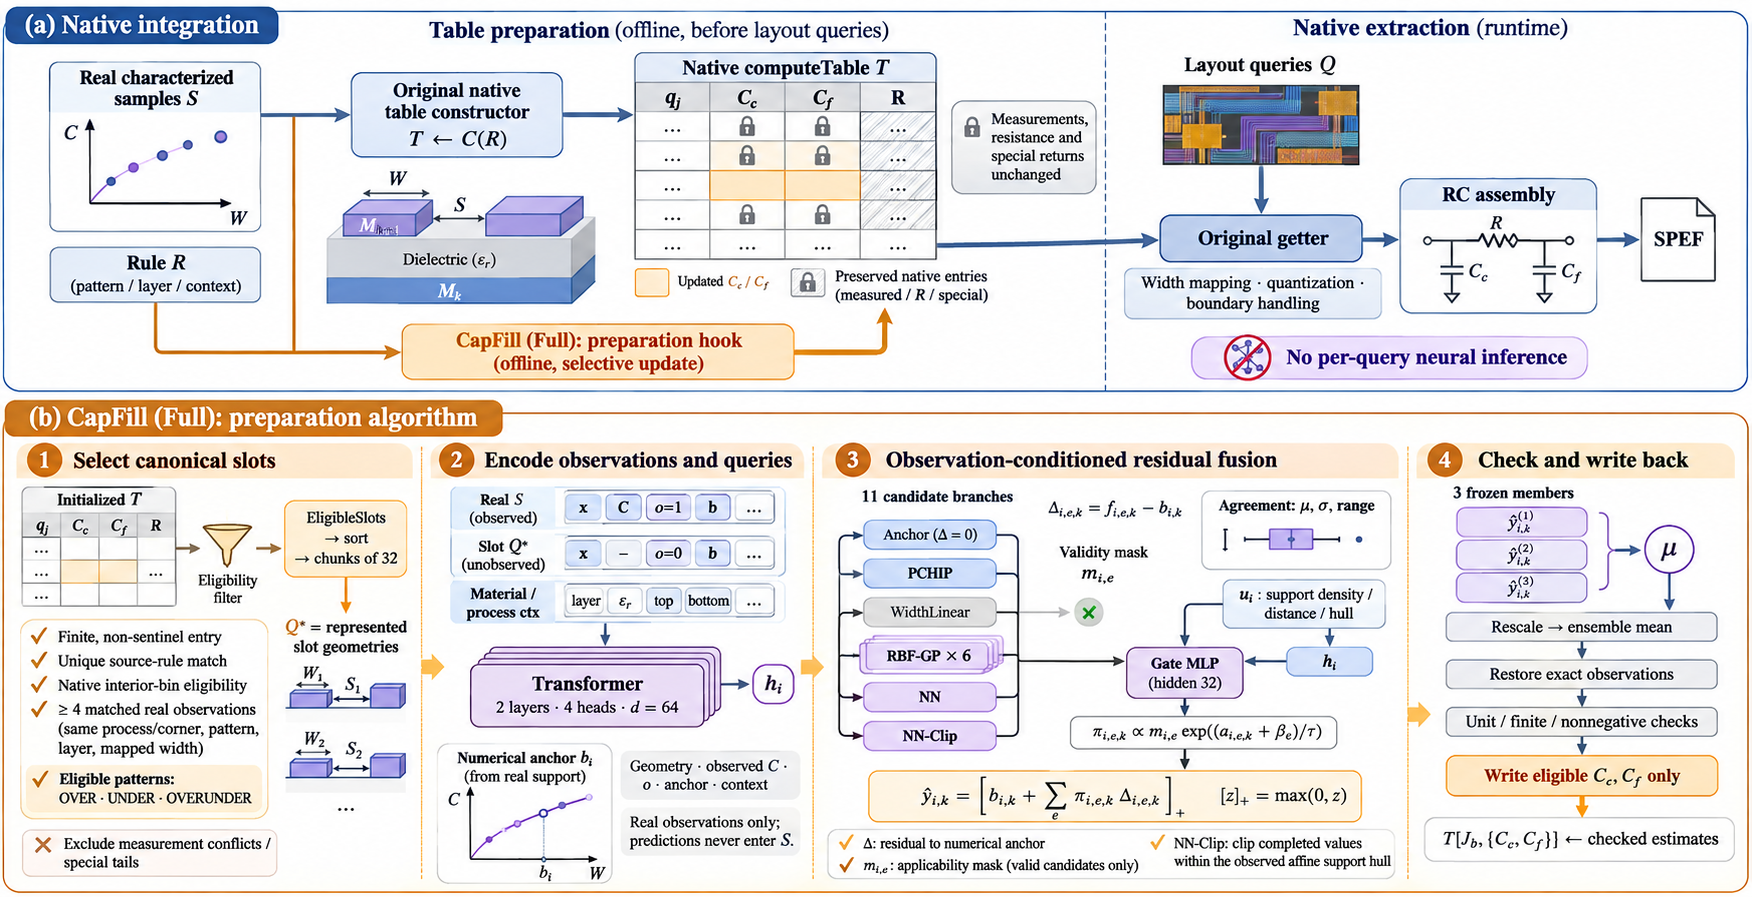
\includegraphics[width=\textwidth]
{figures/compute_table_interface.png}
\caption{Native compute-table integration of CapFill (Full).
The original constructor generates the native
evaluation structure, after which the preparation
hook selectively updates eligible coupling and
fringe capacitance entries. Original measurements,
resistance entries, and special return paths are
preserved. Runtime layout queries continue to use
the original getters and parasitic-network assembly.}
\label{fig:interface}
\end{figure*}


\section{CapFill: Capacitance Estimation and Native Integration}
CapFill denotes the overall observation-conditioned learning framework for capacitance estimation under limited characterization. We call its main implementation \emph{Full}: it uses the complete applicable numerical--neural correction dictionary and component-wise residual fusion described below. \emph{Binary} retains only the simplified anchor/neural gate, and \emph{Ungated} adds the neural residual to the anchor without gated fusion. These names identify the evaluated implementations throughout the experimental results, figures, and ablation comparisons. CapFill's estimation objective is distinct from the native compute-table preparation used to deploy its predictions.

\subsection{Input Encoding and Contextual Representation}

Given a characterized rule, let
$\mathcal{X}=\{\mathbf{x}_i\}_{i=1}^{N}$ denote its
candidate geometry coordinates and
$\mathcal{O}\subseteq\{1,\ldots,N\}$ the observed
characterization indices. Each observation has a
$K$-dimensional capacitance vector
$\mathbf{y}_i\in\mathbb{R}^{K}$.
The remaining coordinates form the query set
$\mathcal{Q}=\{1,\ldots,N\}\setminus\mathcal{O}$.
The objective is to estimate capacitances at
unobserved geometries using only the available
characterization samples and process context.

\textbf{Input Encoding.}
We construct each geometric token from normalized
coordinates, process context, observed capacitances,
observation status, and a numerical anchor.
The normalized geometric coordinates are
\begin{equation}
\widetilde{\mathbf{x}}_i
=
\log\left(
\mathbf{1}+\mathbf{x}_i\oslash\mathbf{s}_x
\right),
\end{equation}
where $\mathbf{s}_x$ denotes the source-derived
coordinate scales. The observed capacitance vector
is encoded as
\begin{equation}
\widetilde{\mathbf{y}}_i
=
o_i(\mathbf{y}_i\oslash\mathbf{s}_y),
\qquad
o_i=\mathbb{1}[i\in\mathcal{O}],
\end{equation}
where $\mathbf{s}_y$ contains the source-derived
capacitance scales. The indicator $o_i$ distinguishes
unobserved entries from observed zero-valued
capacitances.

Let $\mathbf{c}$ denote the process and structural
context, including pattern family, metal-layer
identity, adjacent-layer context, and material
descriptors. With the normalized numerical anchor
$\widetilde{\mathbf{b}}_i=\mathbf{b}_i\oslash\mathbf{s}_y$,
the geometric token is
\begin{equation}
\mathbf{f}_i^{\mathrm{geo}}
=
[
\widetilde{\mathbf{x}}_i;
\mathbf{c};
\widetilde{\mathbf{y}}_i;
o_i;
\widetilde{\mathbf{b}}_i;
\mathbf{t}_{\mathrm{geo}}
],
\label{eq:input_token}
\end{equation}
where $\mathbf{t}_{\mathrm{geo}}=[1,0]$ identifies
a geometric token. Material tokens encoding layer
boundaries and relative permittivity are appended
when available, with $\mathbf{t}_{\mathrm{mat}}=[0,1]$.
Their observation and anchor channels are zero-filled.

\textbf{Contextual Representation.}
The concatenated token sequence
$\mathbf{F}$ is projected into a $d$-dimensional
embedding and processed by a Transformer encoder:
\begin{equation}
\mathbf{H}^{(0)}
=
\mathbf{F}\mathbf{W}_{\mathrm{in}}+\mathbf{b}_{\mathrm{in}},
\qquad
\mathbf{H}^{(L)}
=
\operatorname{Transformer}_{\theta}
(\mathbf{H}^{(0)},\mathbf{M}_{\mathrm{pad}}),
\label{eq:context_encoder}
\end{equation}
where $\mathbf{M}_{\mathrm{pad}}$ masks padded tokens.
We use $L=2$ layers, four attention heads, and
$d=64$ hidden dimensions. The contextual
representation of query $i$ is
\begin{equation}
\mathbf{h}_i=\mathbf{H}^{(L)}_i
\in\mathbb{R}^{d}.
\label{eq:context_embedding}
\end{equation}
The resulting representation captures the
relationships among observed geometries, queries,
and material context, and is shared by the residual
prediction and gating modules.


\subsection{Observation-Conditioned Residual Gating}

Full combines a numerical anchor with
classical and learned correction candidates.
A component-wise gating network determines their
contributions according to the contextual
representation, support geometry, and candidate
agreement.

\textbf{Numerical Anchor and Correction Basis.}
For query $\mathbf{x}_i$, let $b_{i,k}$ denote the
numerical anchor for capacitance component $k$.
It is obtained through piecewise-linear interpolation
for rank-one support, simplex interpolation within
higher-rank support, and nearest-observation fallback
outside the higher-rank interpolation hull or under
degenerate configurations.

We construct a correction dictionary
\begin{equation}
\mathcal{E}=
\{
\mathrm{Anchor},
\mathrm{PCHIP},
\mathrm{WidthLinear},
\mathrm{GP}_{\ell,\lambda},
\mathrm{NN},
\mathrm{NN\text{-}Clip}
\},
\label{eq:correction_basis}
\end{equation}
where $\ell\in\{0.5,1,2\}$ and
$\lambda\in\{10^{-6},10^{-4}\}$ define six
RBF-GP configurations. PCHIP and width-aligned
interpolation are activated only when their
support requirements are satisfied.

Each applicable candidate is represented by its
correction relative to the common anchor:
\begin{equation}
\Delta_{i,e,k}=f_{i,e,k}-b_{i,k},
\qquad
\Delta_{i,\mathrm{Anchor},k}=0,
\label{eq:correction}
\end{equation}
where $f_{i,e,k}$ denotes the candidate prediction.
A validity indicator $m_{i,e}\in\{0,1\}$ identifies
whether candidate $e$ is applicable to query $i$.
The complete dictionary contains eleven candidate
branches, including the anchor and two neural
corrections.

\textbf{Neural Residual and Agreement-aware Gating.}
The Transformer representation is mapped to a
neural residual through a linear prediction head:
\begin{equation}
\Delta_{i,\mathrm{NN},k}
=
\mathbf{w}_k^{\mathsf T}\mathbf{h}_i
+b_k^{\mathrm{NN}}.
\label{eq:neural_residual}
\end{equation}
An additional envelope-clipped residual is defined as
\begin{equation}
\Delta_{i,\mathrm{NN\text{-}Clip},k}
=
\begin{cases}
\operatorname{clip}
(b_{i,k}+\Delta_{i,\mathrm{NN},k},
L_{i,k},U_{i,k})-b_{i,k},
& \mathbf{x}_i\in\Omega,\\
\Delta_{i,\mathrm{NN},k},
& \mathbf{x}_i\notin\Omega,
\end{cases}
\label{eq:clipped_residual}
\end{equation}
where $\Omega$ denotes the characterized support
hull and $L_{i,k},U_{i,k}$ are the corresponding
component-wise envelope bounds.

To characterize candidate agreement, we calculate
the mean, standard deviation, and range of valid
corrections:
\begin{align}
\mu_{i,k}
&=
\frac{1}{N_i}
\sum_{e\in\mathcal{E}}
m_{i,e}\Delta_{i,e,k},\\
\sigma_{i,k}
&=
\sqrt{
\frac{1}{N_i}
\sum_{e\in\mathcal{E}}
m_{i,e}(\Delta_{i,e,k}-\mu_{i,k})^2
+\epsilon
},\\
r_{i,k}
&=
\max_{e:m_{i,e}=1}\Delta_{i,e,k}
-
\min_{e:m_{i,e}=1}\Delta_{i,e,k},
\end{align}
where $N_i=\sum_{e\in\mathcal{E}}m_{i,e}$ and
$\epsilon=10^{-12}$. The gating input combines
these statistics with the contextual representation
and label-blind support descriptors:
\begin{equation}
\mathbf{v}_i=
[
\mathbf{h}_i;
\mathbf{u}_i;
\phi(\boldsymbol{\mu}_i);
\phi(\boldsymbol{\sigma}_i);
\phi(\mathbf{r}_i)
],
\qquad
\phi(z)=\operatorname{sign}(z)\log(1+|z|),
\label{eq:gating_input}
\end{equation}
where $\mathbf{u}_i$ contains support density,
nearest-observation distance, local span,
hull membership, support-region indicators,
affine rank, width validity, coordinate coverage,
and local variation, slope, and curvature features.

A two-layer MLP generates candidate-specific
logits with a hidden dimension of 32:
\begin{equation}
\mathbf{a}_i
=
\mathbf{W}_{g,2}
\operatorname{ReLU}
(\mathbf{W}_{g,1}\mathbf{v}_i+\mathbf{b}_{g,1})
+\mathbf{b}_{g,2}.
\label{eq:gating_logits}
\end{equation}
The logits are combined with learnable candidate
priors $\beta_e$ and a learnable temperature
$\tau=\operatorname{softplus}(\theta_\tau)+10^{-3}$.
The component-wise gating weights are obtained by
a validity-masked softmax:
\begin{equation}
\pi_{i,e,k}
=
\frac{
m_{i,e}\exp((a_{i,e,k}+\beta_e)/\tau)
}{
\sum_{j\in\mathcal{E}}
m_{i,j}\exp((a_{i,j,k}+\beta_j)/\tau)
}.
\label{eq:gating_weights}
\end{equation}
The anchor and neural branches are initialized
without prior suppression, whereas classical
non-anchor corrections start with a negative
logit offset.

\textbf{Residual Fusion.}
The final capacitance estimate is obtained by
fusing the anchor with the weighted corrections:
\begin{equation}
\widetilde{y}_{i,k}
=
b_{i,k}
+
\sum_{e\in\mathcal{E}}
\pi_{i,e,k}\Delta_{i,e,k}.
\end{equation}
To enforce non-negative capacitance, the output
is projected onto the non-negative domain:
\begin{equation}
\widehat{y}_{i,k}
=
\left[
b_{i,k}
+
\sum_{e\in\mathcal{E}}
\pi_{i,e,k}\Delta_{i,e,k}
\right]_{+},
\qquad
[z]_{+}=\max(0,z).
\label{eq:final_prediction}
\end{equation}
All predictions are represented in source-normalized
units and are converted back to physical units
using $\mathbf{s}_y$.


\subsection{Native Compute-Table Population}

CapFill is integrated into OpenRCX's pattern-based
extraction flow by preparing estimated capacitances
in eligible native compute-table entries.
The original compute-table constructor, runtime
getters, and downstream parasitic-network assembly
are retained.

\textbf{Compute-Table Preparation.}
Let $\mathcal{T}$ denote the native distance
compute table constructed for rule descriptor
$\mathcal{R}$. Each table slot $j$ is associated
with a represented geometry coordinate
$\mathbf{q}_j$ and a composite key containing
process/corner, rule identity, pattern family,
routing layers, mapped width, slot index,
separation, output components, and units.

The eligible slot set is
\begin{equation}
\mathcal{J}
=
\left\{
j\in\mathcal{T}:
\begin{array}{l}
j\text{ is finite and non-sentinel},\\
j\text{ has a unique source-rule match},\\
j\text{ belongs to an eligible pattern family}
\end{array}
\right\},
\label{eq:eligible_slots}
\end{equation}
where the eligible families are OVER, UNDER,
and OVERUNDER. Measurement-bin collisions,
special tails, unsupported paths, and resistance
entries are excluded. Original measurement values
and native measure-table return paths remain
unchanged.

Predictions are evaluated at the coordinates
represented by the eligible slots, rather than
at arbitrary runtime requests. The original
characterization support is retained throughout
preparation. Generated values are never reused
as observations.

\textbf{Population and Native Evaluation.}
Algorithm~\ref{alg:compute_table_population} summarizes
the preparation procedure. The eligible slots
are processed in deterministic coordinate order
using query chunks of 32. Only coupling and
fringe capacitance fields are updated. Resistance,
original characterization entries, and special
returns remain native.

\begin{algorithm}[t]
\caption{CapFill Native Preparation with Full}
\label{alg:compute_table_population}
\SetInd{0.35em}{0.5em}
\SetAlgoHangIndent{0.6em}
\Input{Rule $\mathcal{R}$, real samples $\mathcal{S}$, frozen members
$\{F_{\theta^{(m)}}\}_{m=1}^{3}$, scales $(\mathbf{s}_x,\mathbf{s}_y)$, and native constructor $\mathcal{C}$}
\Output{Prepared native compute table $\mathcal{T}$}
$\mathcal{T}\leftarrow\mathcal{C}(\mathcal{R})$\;
$\mathcal{J}\leftarrow\operatorname{SortByCoordinate}(\operatorname{EligibleSlots}(\mathcal{T},\mathcal{R},\mathcal{S}))$\;
\While{$\mathcal{J}\ne\emptyset$}{
 $\mathcal{J}_b\leftarrow\operatorname{TakeNext}(\mathcal{J},32)$\;
 $\mathcal{Q}_b\leftarrow(\mathbf{q}_j)_{j\in\mathcal{J}_b}$\;
 $(\mathbf{F}_b,\mathcal{D}_b,\mathcal{I}_b,\mathbf{M}_{\rm pad})\leftarrow\operatorname{Encode}(\mathcal{S},\mathcal{Q}_b,\mathcal{R},\mathbf{s}_x,\mathbf{s}_y)$\;
 \ForEach{frozen member $m=1,2,3$ (eval mode)}{
  $\mathbf{H}_b\leftarrow\operatorname{Transformer}_{\theta^{(m)}}(\mathbf{F}_b\mathbf{W}_{\rm in}+\mathbf{b}_{\rm in},\mathbf{M}_{\rm pad})$\;
  \ForEach{$i\in\operatorname{Unique}(\mathcal{I}_b)$}{
   $\mathbf{b}_i\leftarrow\operatorname{Anchor}(\mathcal{D}_b,i)$\;
   $(\boldsymbol{\Delta}_i,\mathbf{m}_i,\mathbf{u}_i)\leftarrow\operatorname{ResidualBasis}_{\theta^{(m)}}(\mathbf{H}_b[i],\mathcal{D}_b,i)$\;
   $(\boldsymbol{\mu}_i,\boldsymbol{\sigma}_i,\mathbf{r}_i)\leftarrow\operatorname{Agreement}(\boldsymbol{\Delta}_i,\mathbf{m}_i;10^{-12})$\;
   $\mathbf{a}_i\leftarrow\operatorname{Gate}_{\theta^{(m)}}([\mathbf{H}_b[i];\mathbf{u}_i;\phi(\boldsymbol{\mu}_i);\phi(\boldsymbol{\sigma}_i);\phi(\mathbf{r}_i)])$\;
   $\boldsymbol{\pi}_i\leftarrow\operatorname{MaskedSoftmax}_e(\mathbf{a}_i+\boldsymbol{\beta},\mathbf{m}_i,\tau)$\;
   $\widehat{\mathbf{y}}_i^{(m)}\leftarrow[\mathbf{b}_i+\sum_{e\in\mathcal{E}}\boldsymbol{\pi}_{i,e}\odot\boldsymbol{\Delta}_{i,e}]_+$\;
  }
  $\widehat{\mathbf{Y}}_b^{(m)}\leftarrow\operatorname{Rescale}((\widehat{\mathbf{y}}_{i(j)}^{(m)})_{j\in\mathcal{J}_b},\mathbf{s}_y)$\;
 }
 $\widehat{\mathbf{Y}}_b\leftarrow\frac{1}{3}\sum_{m=1}^{3}\widehat{\mathbf{Y}}_b^{(m)}$\;
 $\widehat{\mathbf{Y}}_b\leftarrow\operatorname{RestoreExactObservations}(\widehat{\mathbf{Y}}_b,\mathcal{S},\mathcal{Q}_b)$\;
 $\widehat{\mathbf{Y}}_b^{\rm native}\leftarrow\operatorname{CheckedNativeValues}(\widehat{\mathbf{Y}}_b,\mathcal{R})$\;
 $\mathcal{T}_{\mathcal{J}_b}^{\rm Cc,Cf}\leftarrow\widehat{\mathbf{Y}}_b^{\rm native}[:,\mathrm{Cc,Cf}]$\;
 $\mathcal{J}\leftarrow\mathcal{J}\setminus\mathcal{J}_b$\;
}
\Return{$\mathcal{T}$}\;
\end{algorithm}

\emph{Algorithm operations.}
$\operatorname{EligibleSlots}$ applies (\ref{eq:eligible_slots}) to initialized slots within one process/corner, pattern, layer and mapped-width context, requiring at least four matched real samples, no sentinel tail or measurement-bin conflict, and native interior-bin eligibility. Sorting uses represented separation and then full slot key. Each $\mathbf{q}_j$ gives the slot geometry in model units. $\operatorname{Encode}$ orders unique support tokens before query tokens, appends material tokens, caches scaled support state $\mathcal{D}_b$, and maps slots to query indices $i(j)$ through $\mathcal{I}_b$.

$\operatorname{ResidualBasis}$ assembles Anchor, PCHIP, WidthLinear, six RBF-GPs, NN and NN-Clip. Anchor has zero correction and is always valid. PCHIP requires single-width support, and WidthLinear requires aligned brackets or an exact hit. Nonfinite numerical predictions are masked. NN uses the residual head. NN-Clip clips the completed value to the support envelope only inside the observed affine space and hull, then subtracts the anchor. Both neural masks are valid. Nonfinite corrections become zero.

$\operatorname{Agreement}$ computes valid-only component-wise mean, standard deviation and range. $\operatorname{Gate}$ implements (\ref{eq:gating_input})--(\ref{eq:gating_logits}). The masked softmax sets invalid logits to $-10^9$ before division by $\tau=\operatorname{softplus}(\theta_\tau)+10^{-3}$. All parameters, including priors and temperature, belong to the current frozen member. $\operatorname{CheckedNativeValues}$ converts units and validates finite, nonnegative predictions before writing only eligible coupling/fringe fields. Observations, resistance, special tails and native return paths remain unchanged. The support set $\mathcal{S}$ contains only observations.




The prepared table is subsequently consumed by
the unchanged native getters, which retain
width selection, coordinate mapping, and
compute-grid quantization. Resistance evaluation
and RC-network assembly are unaffected.
We evaluate unmodified extraction, interface-disabled
extraction, native-value pass-through, Full
injection, and Binary injection as an ablation control. A separate trace
build verifies getter values, while the release
build leaves the original getter implementations
unchanged.

The pinned public API defers table loading until
extraction. Therefore, the first inventory
extraction is included in the preparation cost,
rather than treated as a free rule-only operation.
Preparation and native extraction costs are
measured and reported separately.


\section{Experimental Setup}
\label{sec:experimental_setup}
\subsection{Data and training}
Table~\ref{tab:data} summarizes the datasets and source-training budgets. FEM data cover FreePDK15 and ASAP7. Cross-process prediction trains and selects on FreePDK15 and evaluates on ASAP7. The 84 native holdout tables are excluded from source fitting and selection. Learned capacitance estimates average three trained members.

\begin{table}[t]
\centering
\caption{Characterization data and source-training budgets.}
\label{tab:data}
\begingroup
\fontsize{6.5}{7.2}\selectfont
\setlength{\tabcolsep}{1.5pt}\setlength{\arrayrulewidth}{0.25pt}
\renewcommand{\arraystretch}{1.0}
\begin{tabular*}{\columnwidth}{@{\extracolsep{\fill}}|l||c|c|c|}
\hline
\textbf{Data / training} & \textbf{Public} & \textbf{FEM} & \textbf{Transfer}\\\hline
Geometry rank / units & 1 / native/length & 2 / F/m & 2 / F/m\\
Components & coupling, ground & \multicolumn{2}{c|}{lateral, ground, diagonal}\\\hline
Fit/select/confirm tables & 1051/246/340 & 16/24/16 & 8/12/8\\
Fit/confirm nodes & variable & 153/128 & 153/128\\
Budgeted tables & 338 & 16 & 8\\\hline
Full/Binary/Ungated updates & 24k & 12k & 12k\\
MLP / CNP / adapted AC updates & 3k / 3k / -- & 3k / 3k / 3k & 3k / 3k / 3k\\\hline
\end{tabular*}
\par\vspace{2pt}
\parbox{\columnwidth}{\fontsize{6}{6.7}\selectfont The public inventory contains 1,713 tables. Here k denotes 1,000 updates. Full and its Binary/Ungated ablations use matched updates. AC denotes AttentionCap.}
\endgroup
\end{table}

\subsection{Evaluation protocols and baselines}
Coverage sensitivity uses random, block, and boundary masks at 10/30/50/70\% holdout with seeds 11/29/47/71/101 and shared support/query sets across methods. The fixed-query budget study uses $B=4,8$ for public tables and $B=4,8,16,32,64$ for FEM and transfer.

The primary baselines are the OpenRCX kernel and specified MLI. MLI-ext. adds support-only sparse completion. Numerical controls include Anchor, source-validation-selected GP, affine interpolation, PCHIP, and IDW. Full is CapFill's main implementation. Its matched ablation Binary retains only anchor/neural fusion, whereas Ungated adds the neural residual to the anchor without gating. The ablations share Full's source-training pools, update budgets, and ensemble size. MLP and adapted AttentionCap~\cite{attentioncode} use 200 and 50 support-fitting steps, respectively, selected on source validation. CNP conditions directly on support. AttentionCap retains its Transformer/symmetric head and supervises the same three capacitance components.

Independent FEM evaluation uses 71 layout-parameterized templates from six ASAP7 M4/M5 contexts, with 153 characterization samples per context. Logged widths and spacings define symmetric equal-width side conductors, finite grounded planes, and an exterior grounded boundary. Support and query geometries share materials and boundary conditions. Maxwell matrices provide ground and summed lateral capacitance in F/m.

Native extraction uses AES and Ibex on ASAP7, GF180, IHP SG13G2, and Sky130HS with OpenROAD \texttt{0b54bb3203} and fixed layouts, libraries, and constraints. Compute-table population uses full characterization. Rule-export fidelity compares MLI-ext., the OpenRCX kernel, and Full at $B=4/8$ with shared farthest-point support and seeds 11/29/47. Each budget is capped by the number of available candidates. The 83 eligible held-out tables are completed, with other tables retained. Rule-export timing uses $B=8$ and seed 11. Full-rule extraction supplies the reference for net-capacitance and timing fidelity.

\subsection{Runtime measurement setup}
Direct predictor and resident FEM measurements use one pinned Xeon Gold 6530 CPU thread. Warm predictor evaluation uses three warmups and 20 interleaved blocks, with separate latency and accuracy evaluations for $Q=1,8,32$. Target fitting uses only the observed support, with fitting costs aggregated across six contexts. Native extraction and rule-table preparation are timed separately under their respective deployment protocols.

\subsection{Metrics}
We use $E_g=\sqrt{\sum_{i\in Q_g}(\widehat y_i-y_i)^2/\sum_{i\in Q_g}y_i^2}$ for component group $g$. Groups with nonzero reference energy enter the macro-average. Coverage scores average process/family/component groups and then masks. Physical scores average family/component groups. Fixed-query budget scores pool data seeds before group normalization. Support-protocol scores average member-wise, group-balanced errors. Preparation and native extraction costs are timed separately.

\section{Results}
\subsection{All four characterization holdouts}
\begin{figure*}[t]
\centering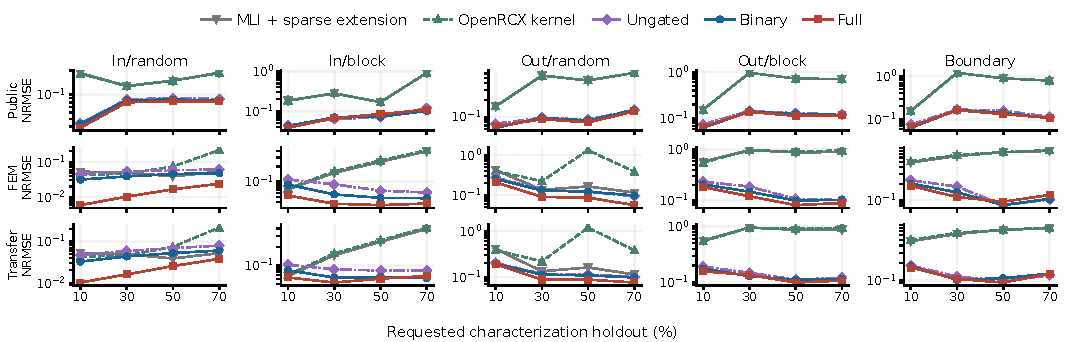
\includegraphics[width=\textwidth]{figures/coverage_four_ratios.pdf}
\caption{Coverage sensitivity: all 10/30/50/70\% holdouts, three domains and five support/protocol conditions. Curves show mean-mask macro NRMSE on common feasible S/Q. Full and its Ungated/Binary ablations each average three matched members. MLI-ext. identifies the specified core plus declared sparse-support/boundary extension. No curve uses the native census to set holdout. Complete-cell coverage, rounded duplicates and full numerical controls are reported separately.}
\label{fig:coverage}
\end{figure*}
Figure~\ref{fig:coverage} includes all 60 domain--holdout--condition cells. Full has lower error than the OpenRCX kernel, MLI with the explicit extension, and Binary in 60, 60, and 49 cells, respectively. The kernels share 21,840/21,840 feasible support/query episodes. Complete MLI cells cover 20.7\% of requested queries across the sweep. The remaining queries use the declared boundary or sparse-support extension. The inventory flags 11,245 repeated rounded S/Q episodes rather than treating them as additional independent evidence. Detailed cells and all numerical controls are retained in the expanded tables.


Across the complete 60-condition sweep, Full, Binary, and Ungated simultaneously improve over both kernel baselines in 60, 55, and 50 conditions, respectively. Full has lower error than Binary in 49 conditions and Ungated in 55, leaving 11 and five local wins for the simplified variants. The default choice is therefore supported by Full's more consistent improvement over the two baselines across evaluated domains, support regions, and missingness patterns, while retaining these local advantages. These results do not imply that a larger gate improves every condition.

\subsection{Task-specific interpolation under fixed budgets}
Field-solver surrogates learn geometry-to-capacitance mappings, whereas capacitance estimation from sparse characterization must use the observed response of the current process. We evaluate this distinction with identical observed geometries and sealed queries, pooling three data seeds before group normalization. Full keeps its learned parameters fixed. Adapted AttentionCap retains its geometry/material Transformer and symmetric head and fits the target capacitance components using the same support~\cite{attentioncap,attentioncode}. Figure~\ref{fig:budget_controls} reports the fixed-budget comparisons.

\begin{figure}[t]
\centering
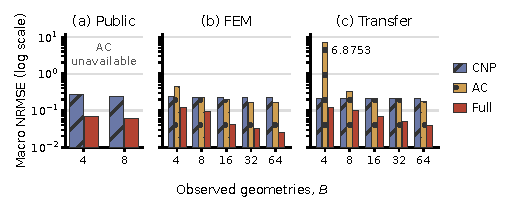
\includegraphics[width=\columnwidth]{figures/fixed_budget_controls.pdf}
\caption{Fixed-budget comparison of CNP, component-supervised adapted AttentionCap (AC), and Full. Pooled-replicate macro NRMSE (log scale, lower is better) on the same $B$ observed geometries and sealed queries. Public evaluations use $B=4/8$ and omit AC because its adapted results are unavailable there. Transfer targets ASAP7.}
\label{fig:budget_controls}
\end{figure}

Full outperforms CNP in all 12 available domain--budget settings and adapted AttentionCap in all ten FEM/transfer settings. On FEM, increasing $B$ from 4 to 64 reduces Full's error from 0.1233 to 0.0250, compared with 0.4546 to 0.1657 for adapted AttentionCap. On transfer, the corresponding errors are 0.1182 to 0.0386 for Full and 6.8753 to 0.1791 for adapted AttentionCap. Public Full achieves 0.0708/0.0609 at $B=4/8$, compared with CNP's 0.2650/0.2374.

These comparisons support a representation tailored to characterization-conditioned interpolation. The numerical anchor incorporates the observed target response, while residual fusion combines source-trained corrections with applicable support-derived estimates. The advantage over the adapted matrix predictor shows that geometry-to-matrix modeling does not automatically provide accurate capacitance estimates under sparse characterization. The Ungated ablation further tests the role of fusion: at $B=64$, Full reduces error from 0.0609 to 0.0250 on FEM and from 0.0814 to 0.0386 on transfer.

Target fitting and numerical interpolation remain strong alternatives in specific regimes. At FEM $B=4$, adapted MLP achieves 0.0515 versus Full's 0.1233. On transfer at $B=64$, MLP/GP achieve 0.0264/0.0271 versus Full's 0.0386. The full-support physical controls likewise favor Anchor (0.00451) over direct Full (0.01675). Their complete tables remain in the extended paper. CapFill therefore targets observation-conditioned capacitance estimation under limited characterization. The following subsection evaluates how these estimates affect extraction fidelity, timing fidelity, and native extraction cost.

\subsection{Downstream fidelity and native extraction cost}
At $B=4/8$, Full reduces net-capacitance and worst-slack errors relative to each kernel in all 16 layout--budget settings (Table~\ref{tab:downstream_fidelity}). Against either baseline, TNS deviation decreases in 13 settings and remains zero for both methods in three. The two kernels use the same operators as Figure~\ref{fig:coverage}, evaluated here on one-dimensional rule tables with shared characterization support, and yield similar downstream errors.

\begin{table}[t]
\centering
\caption{Full fidelity and cost on the same eight layouts under distinct rule-export and full-support compute-table protocols.}
\label{tab:downstream_fidelity}\label{tab:deployment}
\begingroup
\fontsize{5.8}{6.5}\selectfont
\setlength{\tabcolsep}{0.75pt}\setlength{\arrayrulewidth}{0.25pt}
\renewcommand{\arraystretch}{1.0}
\newcommand{\layoutspan}[1]{\raisebox{-3.25pt}[0pt][0pt]{#1}}
\begin{tabular*}{\columnwidth}{@{\extracolsep{\fill}}|l|c||rrr|rrr||rrrrr|}
\hline
\multicolumn{2}{|c||}{\textbf{Layout / budget}} & \multicolumn{6}{c||}{\textbf{Rule-export: error reduction (\%)}} & \multicolumn{5}{c|}{\textbf{Full-support compute table}} \\
\cline{3-13}
 & & \multicolumn{3}{c|}{vs. MLI-ext.} & \multicolumn{3}{c||}{vs. OpenRCX} & \multicolumn{5}{c|}{Fidelity and preparation / extraction cost} \\
\cline{3-13}
\textbf{Layout} & $B$ & C & WS & TNS & C & WS & TNS & C err. & Prep. & PEX & SPEF & $T/T_0$ \\
\hline
\layoutspan{\textbf{ASAP7/AES}} & 4 & 81.2 & 89.7 & 84.1 & 81.1 & 89.6 & 84.0 & \layoutspan{0.00426} & \layoutspan{5.41} & \layoutspan{2.05} & \layoutspan{0.49} & \layoutspan{0.991} \\
 & 8 & 89.1 & 88.4 & 89.5 & 89.0 & 88.4 & 89.5 &  &  &  &  &  \\
\hline
\layoutspan{\textbf{ASAP7/IBEX}} & 4 & 81.4 & 90.3 & 85.6 & 81.3 & 90.2 & 85.5 & \layoutspan{0.00516} & \layoutspan{5.41} & \layoutspan{3.30} & \layoutspan{0.72} & \layoutspan{1.020} \\
 & 8 & 89.2 & 98.3 & 96.7 & 89.2 & 98.3 & 96.7 &  &  &  &  &  \\
\hline
\layoutspan{\textbf{GF180/AES}} & 4 & 84.6 & 85.0 & 84.4 & 84.6 & 85.0 & 84.4 & \layoutspan{0.00030} & \layoutspan{8.39} & \layoutspan{2.45} & \layoutspan{0.52} & \layoutspan{1.031} \\
 & 8 & 78.7 & 78.5 & 78.3 & 78.7 & 78.5 & 78.3 &  &  &  &  &  \\
\hline
\layoutspan{\textbf{GF180/IBEX}} & 4 & 84.5 & 85.1 & 84.4 & 84.5 & 85.1 & 84.4 & \layoutspan{0.00020} & \layoutspan{8.39} & \layoutspan{2.73} & \layoutspan{0.52} & \layoutspan{0.999} \\
 & 8 & 78.4 & 78.7 & 77.7 & 78.4 & 78.7 & 77.7 &  &  &  &  &  \\
\hline
\layoutspan{\textbf{IHP/AES}} & 4 & 91.3 & 94.5 & -- & 91.3 & 94.5 & -- & \layoutspan{0.05656} & \layoutspan{13.99} & \layoutspan{2.00} & \layoutspan{0.40} & \layoutspan{1.035} \\
 & 8 & 87.4 & 90.1 & -- & 87.4 & 90.1 & -- &  &  &  &  &  \\
\hline
\layoutspan{\textbf{IHP/IBEX}} & 4 & 92.5 & 93.3 & 100.0 & 92.5 & 93.3 & 100.0 & \layoutspan{0.05477} & \layoutspan{13.99} & \layoutspan{3.10} & \layoutspan{0.66} & \layoutspan{1.029} \\
 & 8 & 87.6 & 88.2 & -- & 87.5 & 88.1 & -- &  &  &  &  &  \\
\hline
\layoutspan{\textbf{Sky130/AES}} & 4 & 89.7 & 94.5 & 97.1 & 89.9 & 94.6 & 97.1 & \layoutspan{0.00382} & \layoutspan{8.48} & \layoutspan{2.43} & \layoutspan{0.56} & \layoutspan{1.017} \\
 & 8 & 87.3 & 83.5 & 76.6 & 87.3 & 83.1 & 76.2 &  &  &  &  &  \\
\hline
\layoutspan{\textbf{Sky130/IBEX}} & 4 & 88.4 & 91.1 & 89.6 & 88.6 & 91.2 & 89.8 & \layoutspan{0.00233} & \layoutspan{8.48} & \layoutspan{2.29} & \layoutspan{0.58} & \layoutspan{1.024} \\
 & 8 & 85.6 & 78.0 & 81.7 & 85.6 & 77.4 & 81.1 &  &  &  &  &  \\
\hline
\end{tabular*}
\par\vspace{2pt}
\parbox{\columnwidth}{\fontsize{6}{6.7}\selectfont Rule-export values average seeds 11/29/47. C denotes capacitance NRMSE. WS/TNS are absolute timing deviations from full-table extraction. ``-- means both errors are zero. Compute table: C err. is net-C NRMSE. Prep./PEX/SPEF are in seconds. $T/T_0$ is the mean extraction ratio over three release runs. Preparation includes inventory and loading. Native table construction/injection stays within PEX. Shared right-hand values use full characterization, not the row budget $B$.}
\endgroup

\end{table}

Against MLI-ext., for GF180/IBEX at $B=8$, capacitance NRMSE decreases from 0.0161 to 0.00348, $|\Delta\mathrm{WS}|$ from 38.25 to 8.14\,ps, and $|\Delta\mathrm{TNS}|$ from 52.74 to 11.77\,ns. Figure~\ref{fig:downstream_spatial} shows both kernel comparisons across four IBEX layouts. Mean endpoint error falls by 77.8--91.1\% relative to either baseline, with improvements in all 12 process--seed pairs for each comparison.

\begin{figure}[t]
\centering
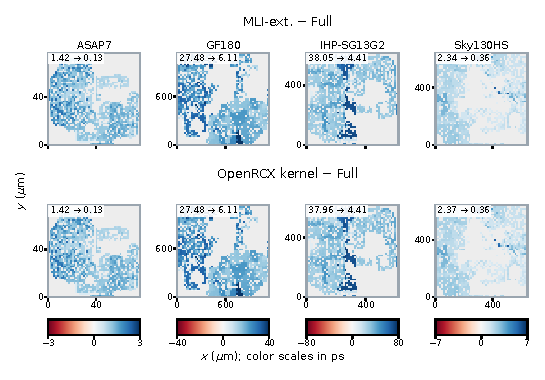
\includegraphics[width=\columnwidth]{figures/downstream_two_kernels.pdf}
\caption{Spatial timing fidelity at $B=8$, four IBEX layouts. Columns: ASAP7, GF180, IHP-SG13G2, Sky130HS. The top row shows MLI-ext. minus Full, and the bottom row shows OpenRCX kernel minus Full. Maps average endpoint absolute-error reductions against full-table extraction over seeds 11/29/47 and $50\times50$ bins. Annotations give baseline$\to$Full MAE (ps). Each column shares a symmetric scale: blue indicates improvement, red degradation, gray empty bins. Coordinates are in $\mu$m.}
\label{fig:downstream_spatial}
\end{figure}

The new interface populates 49,657 eligible finite slots across four rule libraries. Native-value pass-through preserves traced getter returns and electrical SPEF records on all eight layouts. Full changes 924,647 traced returns. Covered returns match injected values, and resistance/uncovered returns remain identical. Table~\ref{tab:deployment} reports the newly measured path: across 120 release runs, the Full extraction/original ratio ranges from 0.991 to 1.035. Including inventory, input/model/support preparation and process-startup residual, first-design PEX overhead ranges from 161.1\% to 670.4\%. SPEF output and STA are measured separately and are not used to dilute this denominator. Values below one are repeat-run variation, not a stable acceleration claim.


Full's net-C fidelity error ranges from 0.00020 to 0.05656. The largest errors occur on IHP, with worst-slack changes of 74.4/147.4\,ps for AES/Ibex. These are deviations from native full-rule extraction, not improvements against an independent field reference.

The fixed-node rule-export configuration has a different support and deployment contract. Across 96 release runs, Full's extraction/original ratio is 0.983--1.047. Four-library B=8 prediction/export costs 0.70/0.67/0.91\,s for MLI-ext./Binary/Full, plus 0.88\,s shared setup. The MLI-ext. timing uses the output-equivalent archived CMI implementation. Full improves net-C and worst-slack fidelity over MLI-ext. in all 16 layout--budget cells, and improves over Binary in six and four cells, respectively. Binary has lower P99 endpoint error in ten. These fidelity and timing results are retained without relabeling them as computeTable injection.

Although Full incurs higher direct inference cost than simpler numerical and learned predictors, its deployment does not require neural inference for individual layout queries. Instead, predictions are generated during rule-table preparation, while native OpenRCX lookup and parasitic-network assembly remain unchanged. Therefore, the proposed method targets improved capacitance and downstream timing fidelity under limited characterization rather than faster online inference. The additional preparation cost is reported separately from native extraction time (Table~\ref{tab:deployment}).

\section{Conclusion}
We presented CapFill, an observation-conditioned framework for capacitance estimation from sparse characterization in pattern-based parasitic extraction. It combines process-specific observations, geometry and material context, and numerical--neural residual corrections to reduce estimation errors that propagate into extraction and timing analysis. Full is the main implementation, with Binary and Ungated as matched ablations. Preparing estimates in native compute tables preserves existing pattern matching, lookup, and parasitic-network assembly.

Full lowers macro NRMSE relative to both kernel baselines in all 60 evaluated coverage conditions, versus 55 for Binary and 50 for Ungated. This consistency supports Full as the unified default while retaining the simplified variants' local advantages. Separate rule-export evaluations improve net-capacitance and worst-slack fidelity in all 16 layout--budget settings. At $B=8$, mean endpoint timing error falls by 77.8--91.1\% across four IBEX layouts relative to either kernel. Numerical interpolation remains more accurate on fully supported physical-reference templates, and native compute-table fidelity is evaluated separately. These results support improved capacitance estimation and downstream fidelity under the assessed characterization budgets and deployment protocols.
\clearpage
\bibliographystyle{IEEEtran}\bibliography{references}
\end{document}
